\documentclass[a4paper,10pt]{article}

%\usepackage{natbib}
\usepackage{amsthm}
\usepackage{amsfonts}
\usepackage{amssymb}
\usepackage{amsmath}
\usepackage{latexsym}
\usepackage{graphicx}
\usepackage{blindtext}

\usepackage{doc}

\newtheorem*{theorem}{Theorem}
\theoremstyle{definition}
\newtheorem*{definition}{Definition}

\hoffset -1in \topmargin 0mm \voffset 0mm \headheight 0mm
\headsep0mm
\oddsidemargin  20mm     %   Left margin on odd-numbered pages.
\evensidemargin 20mm     %   Left margin on even-numbered pages.
\textwidth   170mm       %   Width of text line.
\textheight  252mm

\makeatletter
\renewcommand\@openbib@code{%
     \advance\leftmargin  \z@ %\bibindent
      \itemindent \z@
     % Move bibitems close together
     \parsep -0.8ex
     }
\makeatother

\makeatletter
\renewcommand\section{\@startsection {section}{1}{\z@}%
                                   {-3.5ex \@plus -1ex \@minus -.2ex}%
                                   {1.5ex \@plus.2ex}%
                                   {\large\bfseries}}
\makeatother

\makeatletter
\renewcommand\subsection{\@startsection {subsection}{1}{\z@}%
                                   {-3.5ex \@plus -1ex \@minus -.2ex}%
                                   {1.5ex \@plus.2ex}%
                                   {\normalsize\bfseries}}
\makeatother

\makeatletter
	\setlength{\abovecaptionskip}{3pt}   % 0.25cm 
	\setlength{\belowcaptionskip}{3pt}   % 0.25cm 
\makeatother

\begin{document}
\pagestyle{empty}

\begin{center}
{\bf \Large Industry 4.0 in farming}
\end{center}

\smallskip
\begin{center}
{\large Jakub Eim}
\end{center}

\smallskip
\begin{center}
Faculty of Mechanical Engineering, Brno University of Technology\\
Institute of Automation and Computer Science\\
Technicka 2896/2, Brno 616 69, Czech Republic\\
jakub.eim@vutbr.cz\\
\end{center}

\bigskip
\noindent Abstract: \textit{The Topic of this research paper is the implementation of Industry 4.0 in farming. Newly introduced technology aims at replacing human workers with robots for repetitive tasks like food picking and reducing the number of chemicals needed to harvest enough quality products. }

\vspace*{10pt} \noindent Keywords: \textit{Industry 4.0, Farming, Robotic picker, Robotic weeder, Automatization, Lasers, Robotic arms }

\bigskip
\section{Introduction}
\label{sec:1}

Farming is one of the oldest industries known to humans. But with increasing standards of living it gets harder and harder to find workers willing to do manual farming labour. In combination with the rapidly increasing number of humans inhabiting the earth, using autonomous robots and systems for farming will be essential in the future. This situation introduces major fields of opportunity for automation in the farming industry. The first one is robotic pickers for fruits and vegetables, and the other field to be improved and revolutionized by industry 4.0 is the equipment used for crop farming. Both will be addressed in this research paper.


\bigskip
\section{Traditional farming}
\label{sec:2}

Farming as we know it today has very little automation happening. In the summer, it is human workers picking strawberries, apples, potatoes, etc. On the fields tractors can be seen, many already using GPS navigation. However, to fully embrace the opportunity given by Industry 4.0, the farming industry needs robots \cite{SICILIANO_rhandbook}. capable of strategic thinking via artificial intelligence. Even though technology advances quickly, there are major setbacks in farming preventing automatization, the biggest of which is currently the price of automated types of equipment and robots, making it available only to big farms. Another limitation is the fact that all systems require a reliable power source.

\bigskip

\begin{figure}[h]
\begin{center}
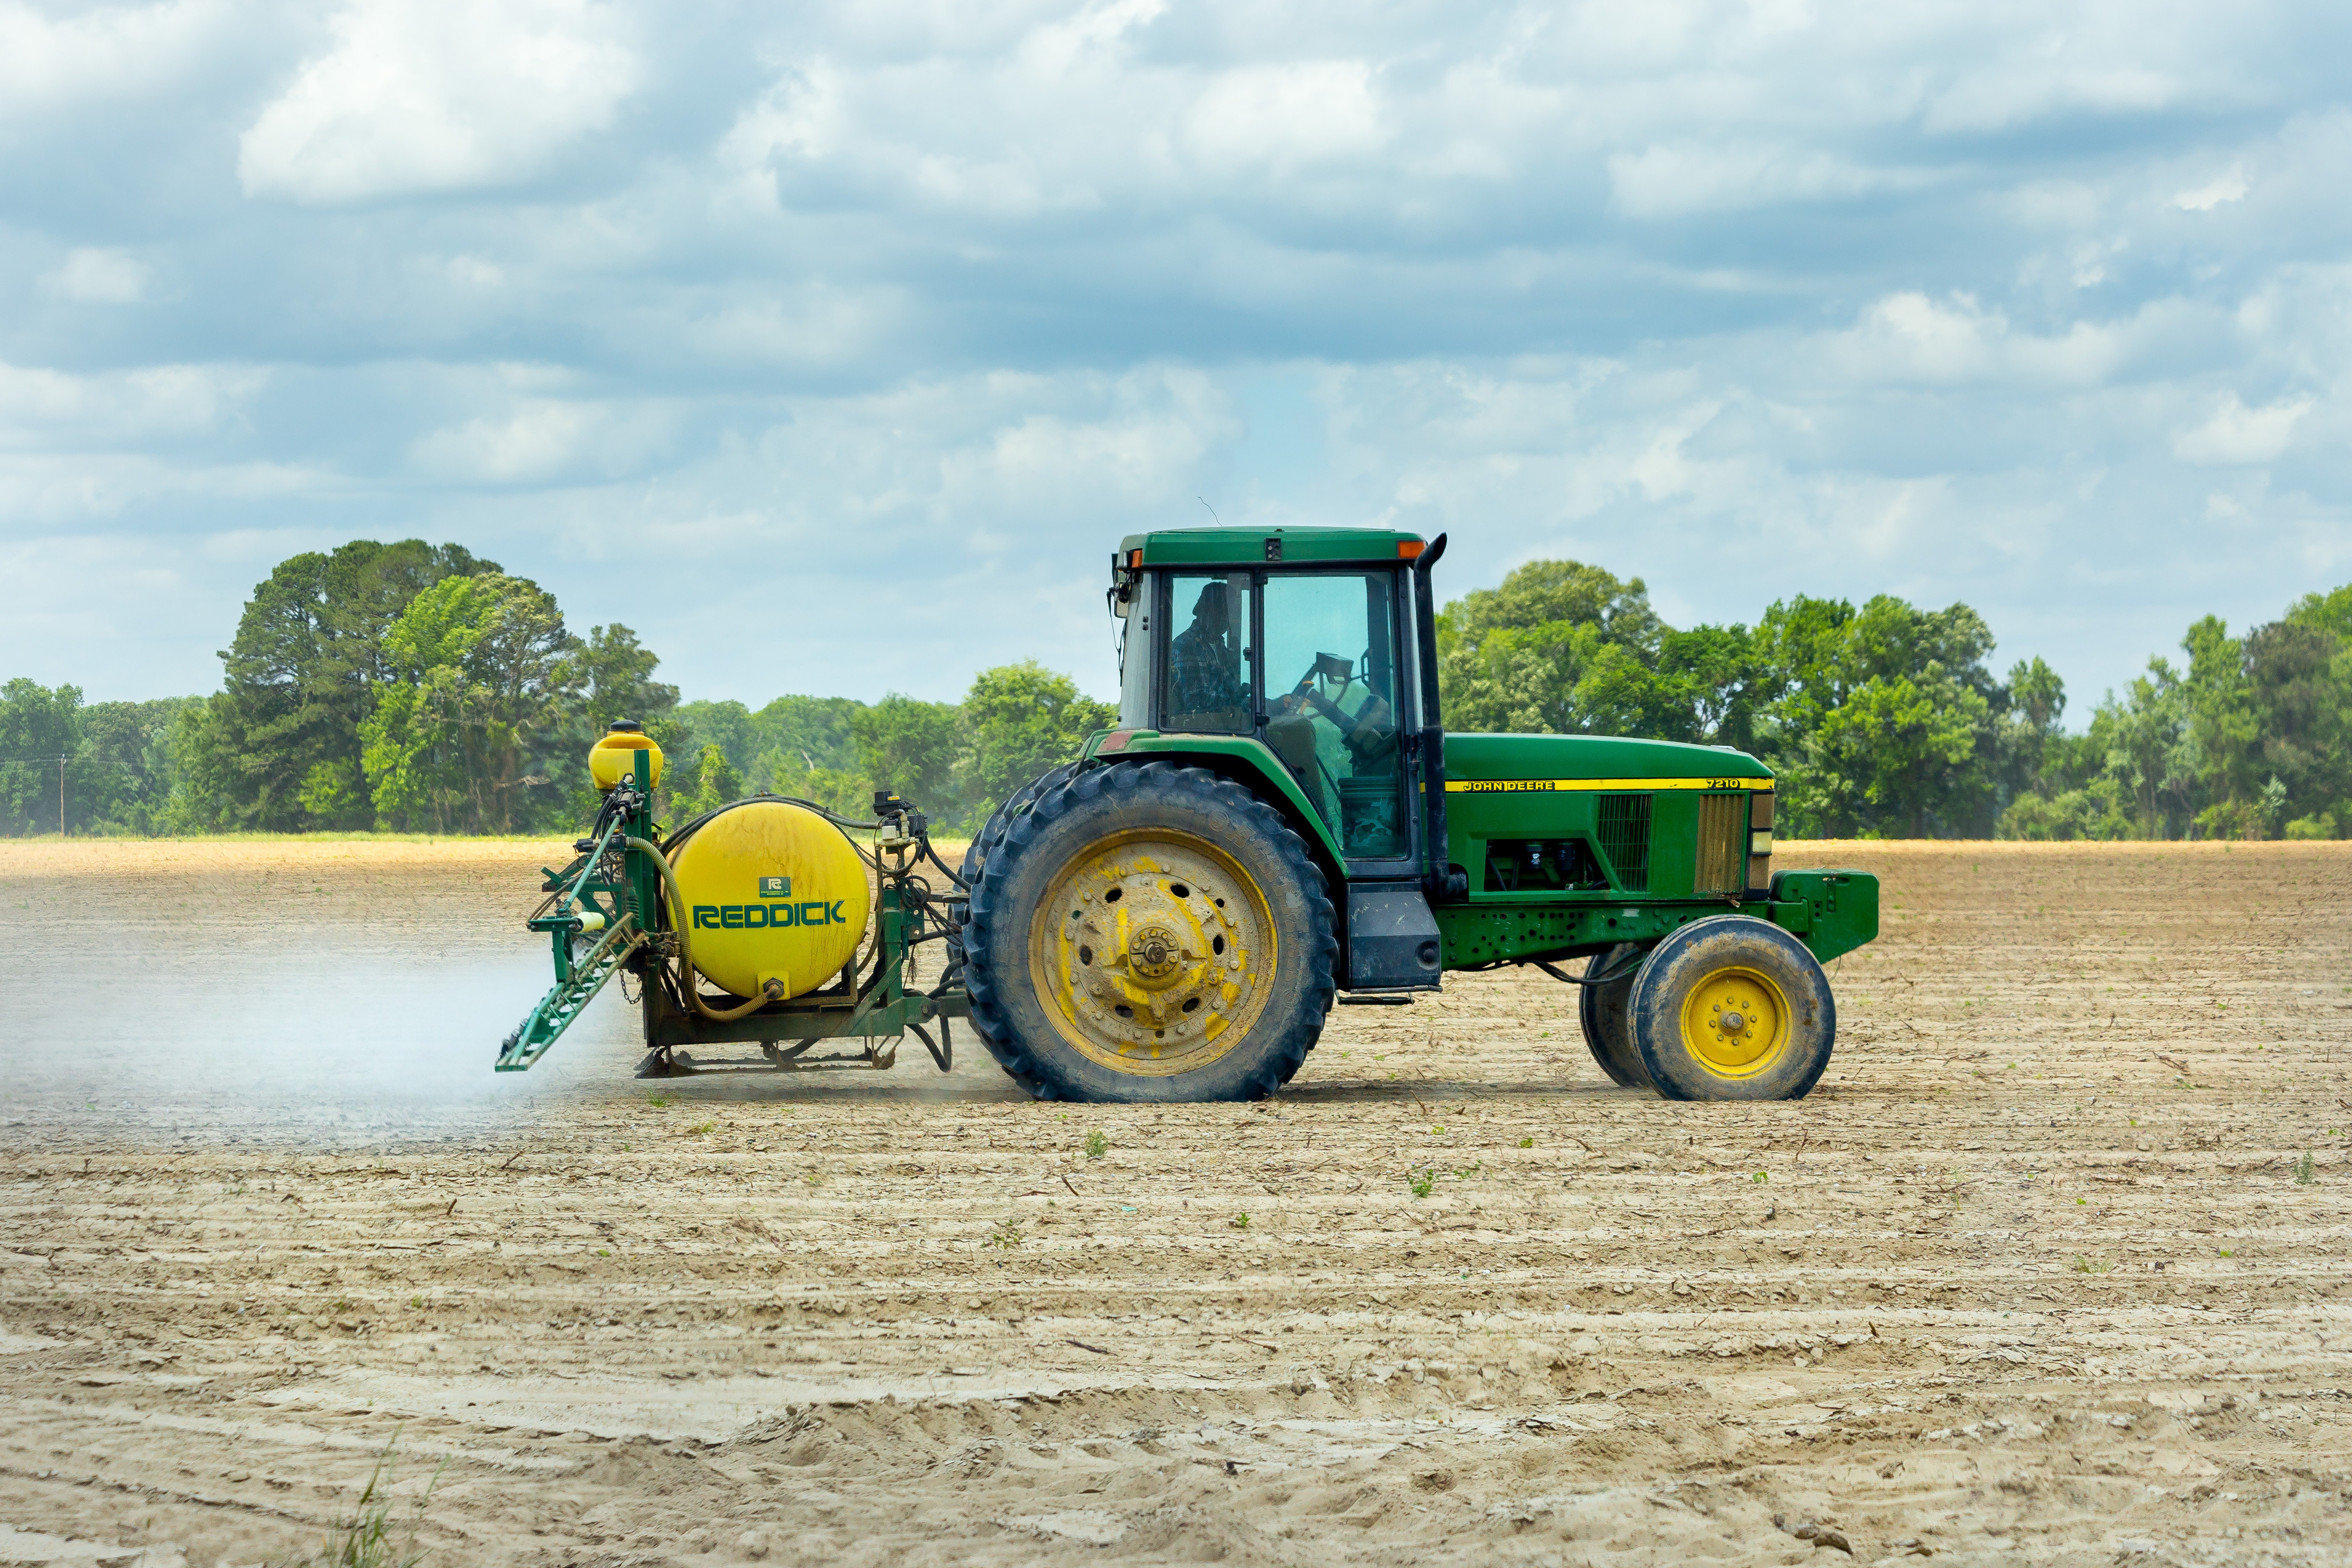
\includegraphics[scale=0.06]{image/traditional_farming.jpg}
\caption{Inefficient traditional crop spraying}
\end{center}
\end{figure}

\newpage

\section{Weeding robots}
\label{sec:3}

Weed control is one of the most important things in farming, with weeds competing for sunlight and resources while reducing yield\cite{9396005}. Today it is done by spraying the ground with a large amount of pesticides and herbicides. By using purely mechanical spraying equipment, the ground is evenly coated in chemicals. Since some areas need more weed control than others, it introduces strategic planning to the proccess\cite{McVLAHpD06ypNajG}. Using high-quality cameras, light, computer vision and artificial intelligence, robots today can scan and create a digital copy of fields containing over 4 million plants. Using the data, the robot then decides which plants to kill and which to fertilize and manure\cite{9798733}. Robots treat each plant or crop individually, saving time and resources on plants growing well with no weeds around. 
\bigskip

\begin{figure}[h]
\begin{center}
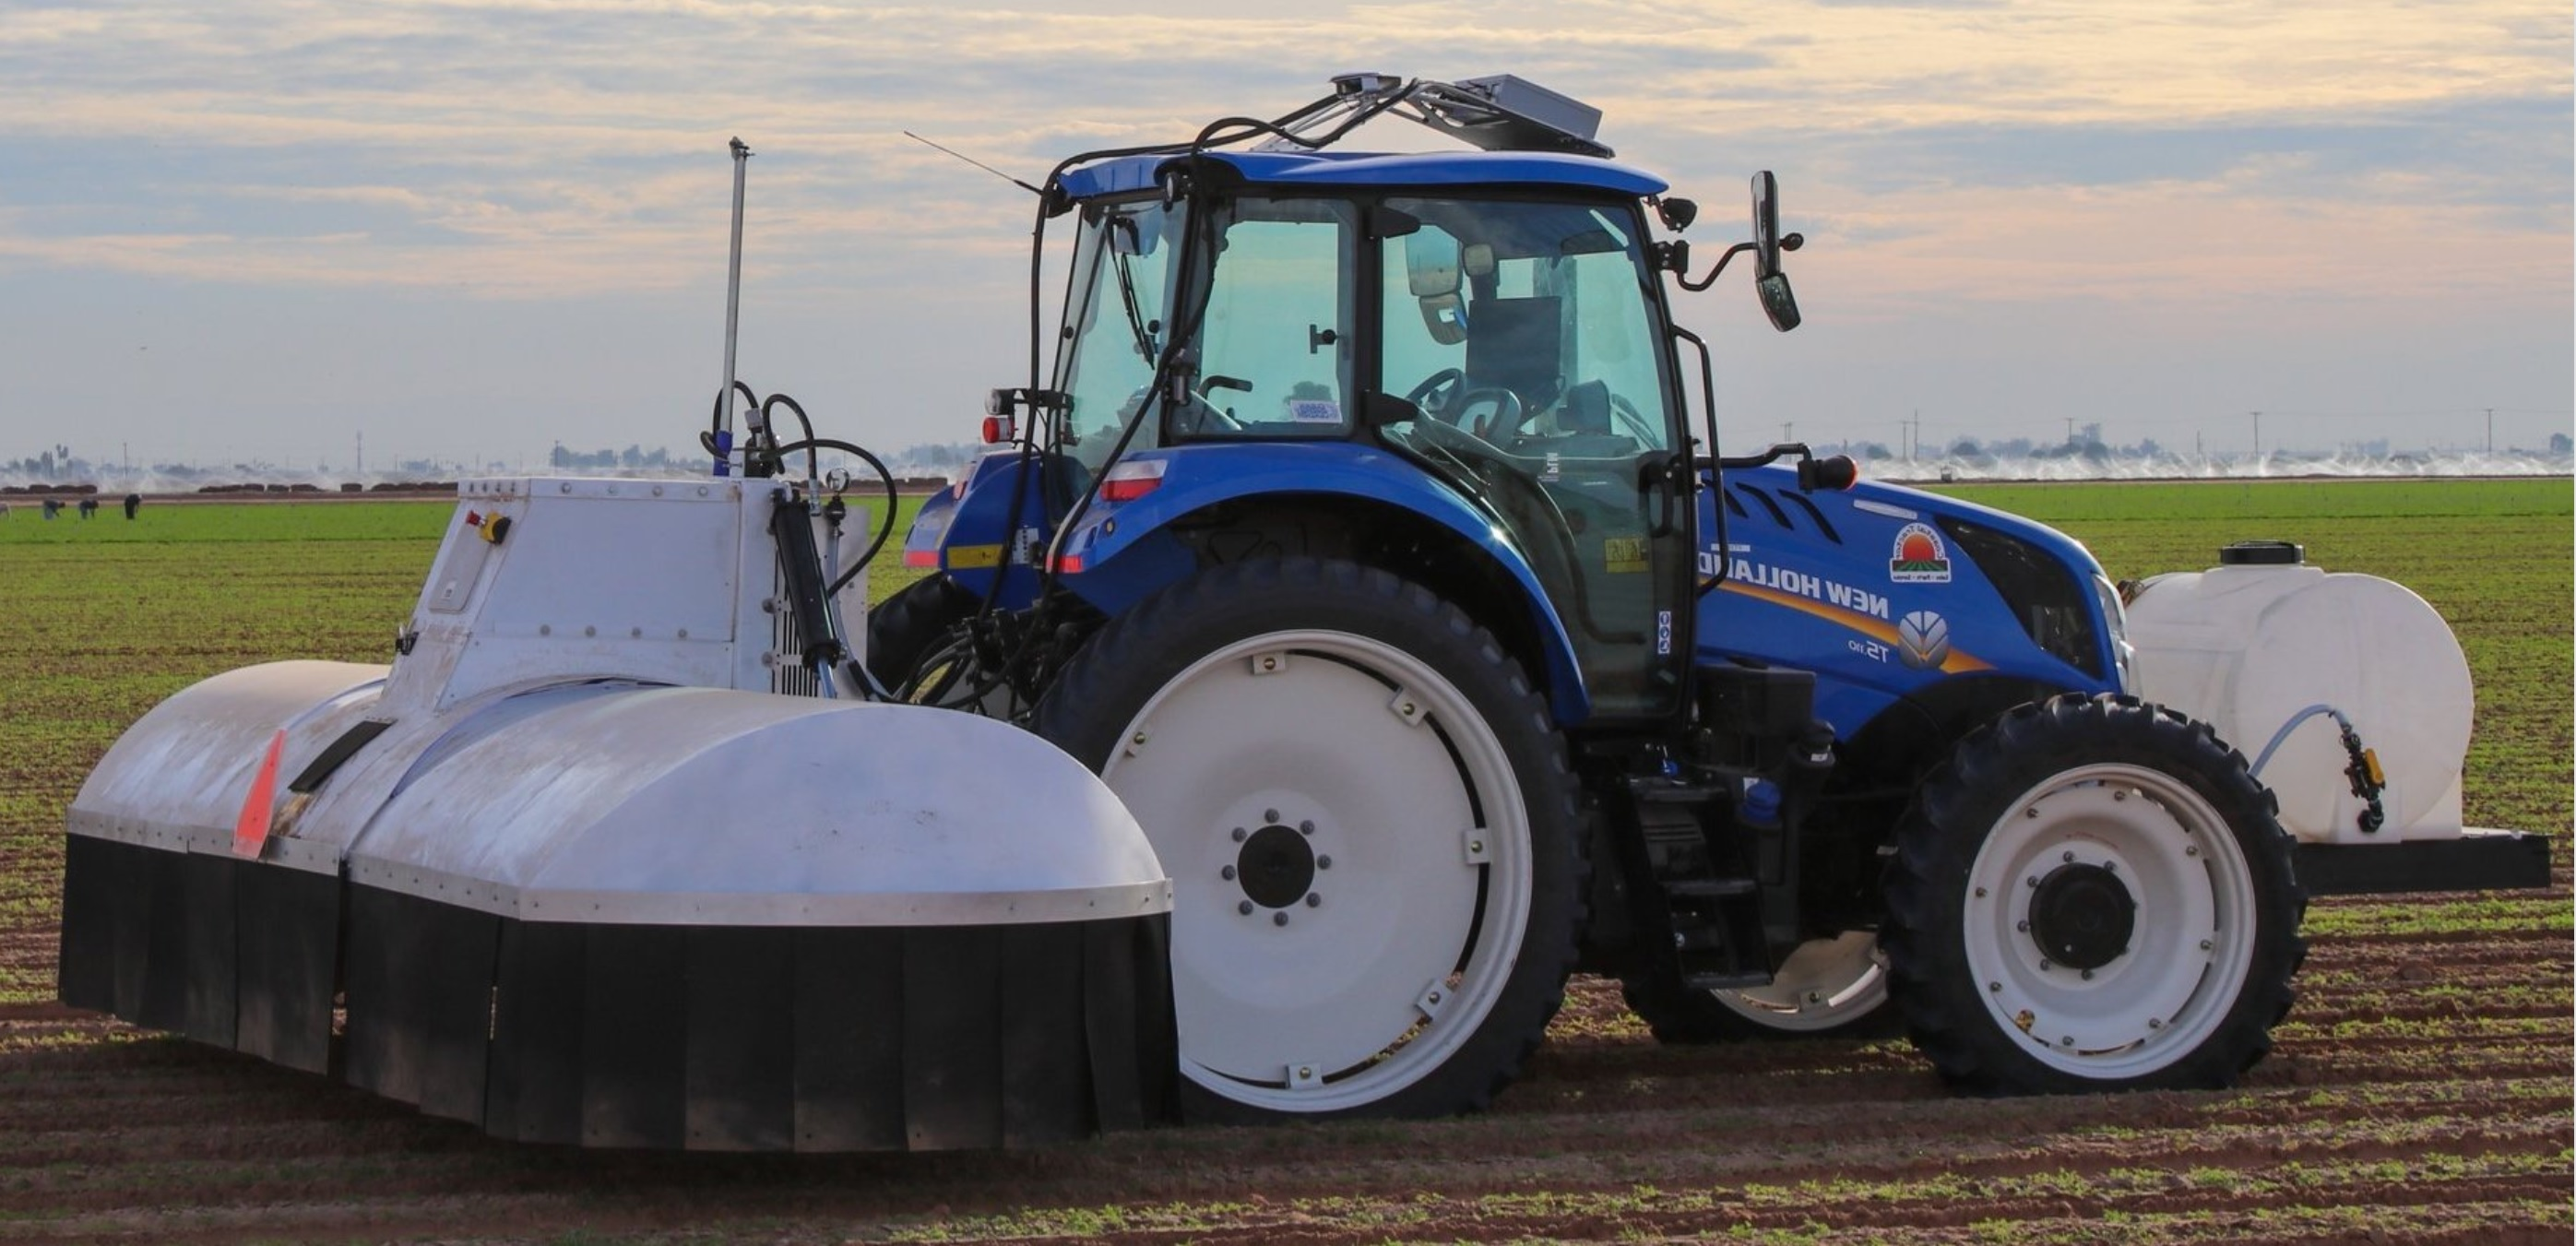
\includegraphics[scale=0.5]{image/verdant_robotics.jpg}
\caption{Verdant robotics weeding equipment \cite{HBFeJBEg5CO6iD1l}}
\label{fig:2}
\end{center}
\end{figure}


\subsection{Robots using pesticides}
\label{subsec:1}

Verdant robotics based in America developed spraying equipment for fertilization and weeding. Using computer vision and machine learning, it can differentiate between produced plants and weeds. This means, that as the machine hovers over the plants, it decides which plant to fertilize and which to kill. Then it shoots the right amount of liquid onto each individual plant \cite{10.1007/978-3-319-47952-1_60}. This requires precision nozzles and positioning considering the fact that fields are often rough 3D terrain. This procedure saves up to 90 \% of fertilizers and pesticides. 

\bigskip

\begin{figure}[h!]
\begin{center}
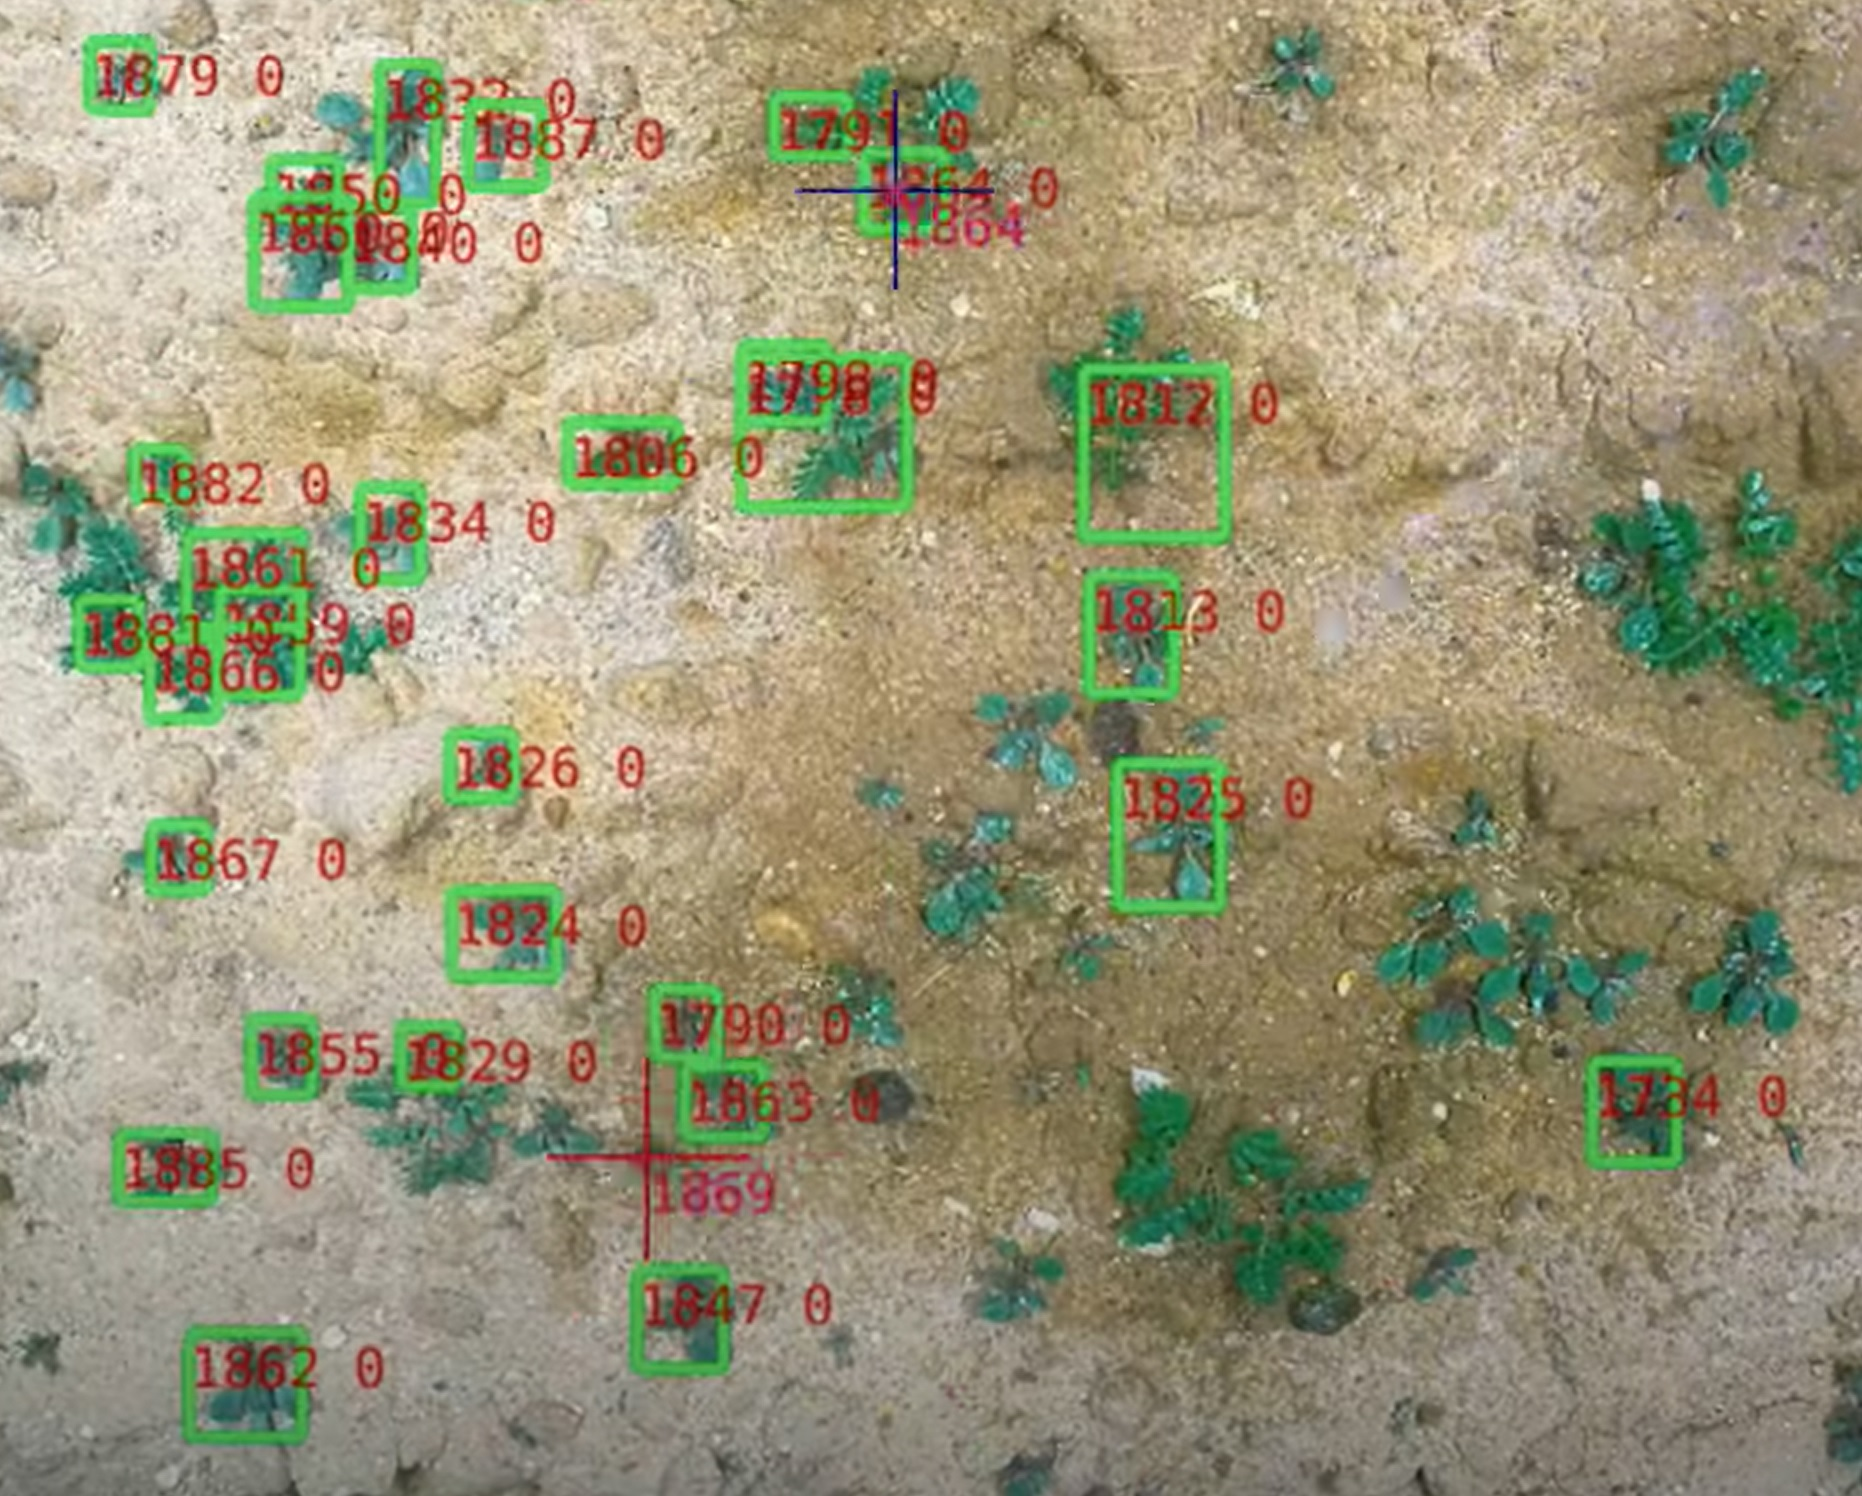
\includegraphics[scale=0.4]{image/verdant_vision.jpg}
\caption{Verdant robotics computer vision \cite{HBFeJBEg5CO6iD1l}}
\end{center}
\end{figure}

\subsection{Robots using lasers}
\label{subsec:2}

While reducing the amount of chemicals during weeding proccess is an improvement, another even more ecological approach is weeding using lasers. The robot made by Carbon robotics itself has many individual weeding modules, consisting of high power LED lights, cameras and 150W lasers that fire weeds 20 times per second. Laser beam is directed at the base of the weed, so there is almost no damage done to the soil. It's biggest limitation is that the lasers are only effective at terminating young weeds, which makes it less suitable for weeding colonies of matured weeds, which isn't a problem for pesticide spraying robots. 

\smallskip

\begin{figure}[h]
\begin{center}
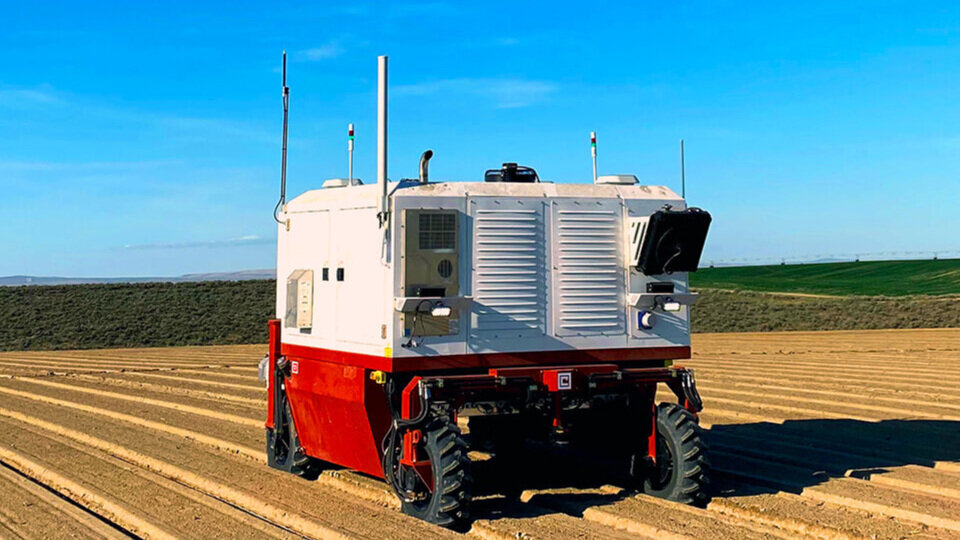
\includegraphics[scale=0.4]{image/carbon_robot.jpg}
\caption{Carbon robotics weeding robot\cite{Swvcwnh6tdQ4SRdV}}
\end{center}
\end{figure}

\smallskip
Similarly, the robot uses cameras and computer vision to address weeds in real-time, which are then targeted by Deep-learning-based computer vision models using artificial intelligence running on Nvidia graphics cards. This ensures precise targeting of the crops to be burned.

\bigskip
\begin{figure}[h]
\begin{center}
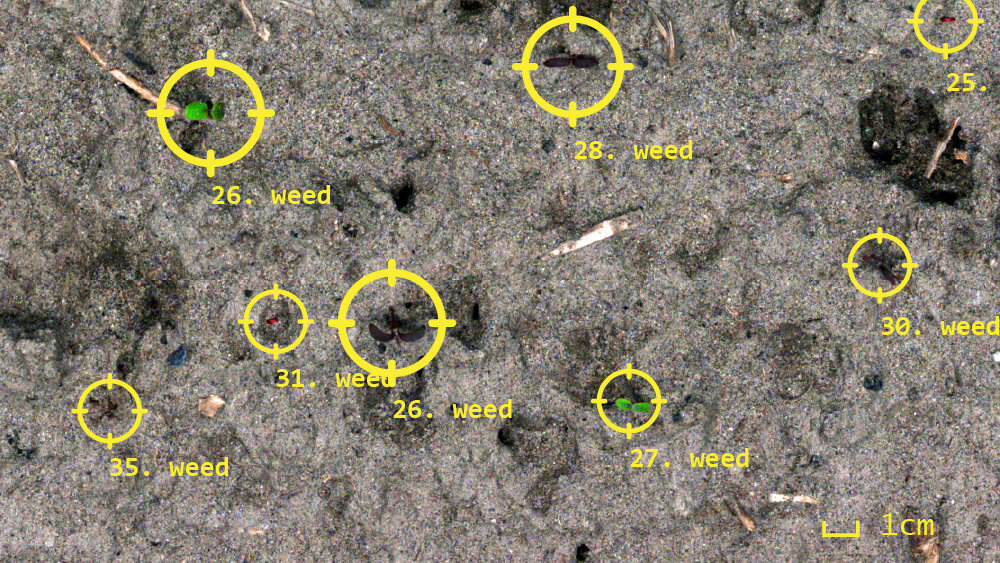
\includegraphics[scale=0.2]{image/carbon_vision.jpg}
\caption{Carbon robotics computer vision with AI targeting \cite{Swvcwnh6tdQ4SRdV}}
\end{center}
\end{figure}

\newpage

\section{Robotic pickers}
\label{sec:4}
Another important part of farming is gathering the produced goods. While many of those are obtained mechanically with no need for human labor, like corn, potatoes, rice, sunflowers, there are many farmed products that currently require manual labour. Industry 4.0 aims at replacing hardworking humans at gathering fruits \& vegetables. Nowadays robots are cabaple of gathering strawberries, tomatoes, apples, and other kind of round-ish food\cite{9675502}. 

\smallskip
\subsection{Dogtooht's robot}
\label{subsec:3}

British company Dogtooth currently sells strawaberry harvesting robot with 6 DOF and track carrier. The robots are equipped with track to cope with muddy incline terrain in which they need to operate. Each robotic picking arm is equipped with LED lights for two cameras that create a 3D image of harvested strwaberies. 3D image is then proccessed and the robot computes the needed vector and angle of the fruit. Since it has 6 DOF with more than 360° of rotation at each joint, it can access the strawaberry from multiple angles. Everything about this robot is made from scratch, no premade robotic arms were used. Each robot has an inspection system in the center, where the strawberries are scanned for 17 types of deffect. Based on the results, they are sorted into coresponding clamshell or laid off for additional inspection by humans. Human inspection is ussualy required if there are multiple strawberries on one stem. Main advantage is that the robot only touches the stem, never the strawberry itself, so there aren't any bruises or mould present on the strawberries. The setback of this robot is that the strawberries have to be farmed at arms height, so one has to account for robotic farming at the beggining of building a strawberry farm. 

\bigskip
\begin{figure}[h]
\begin{center}
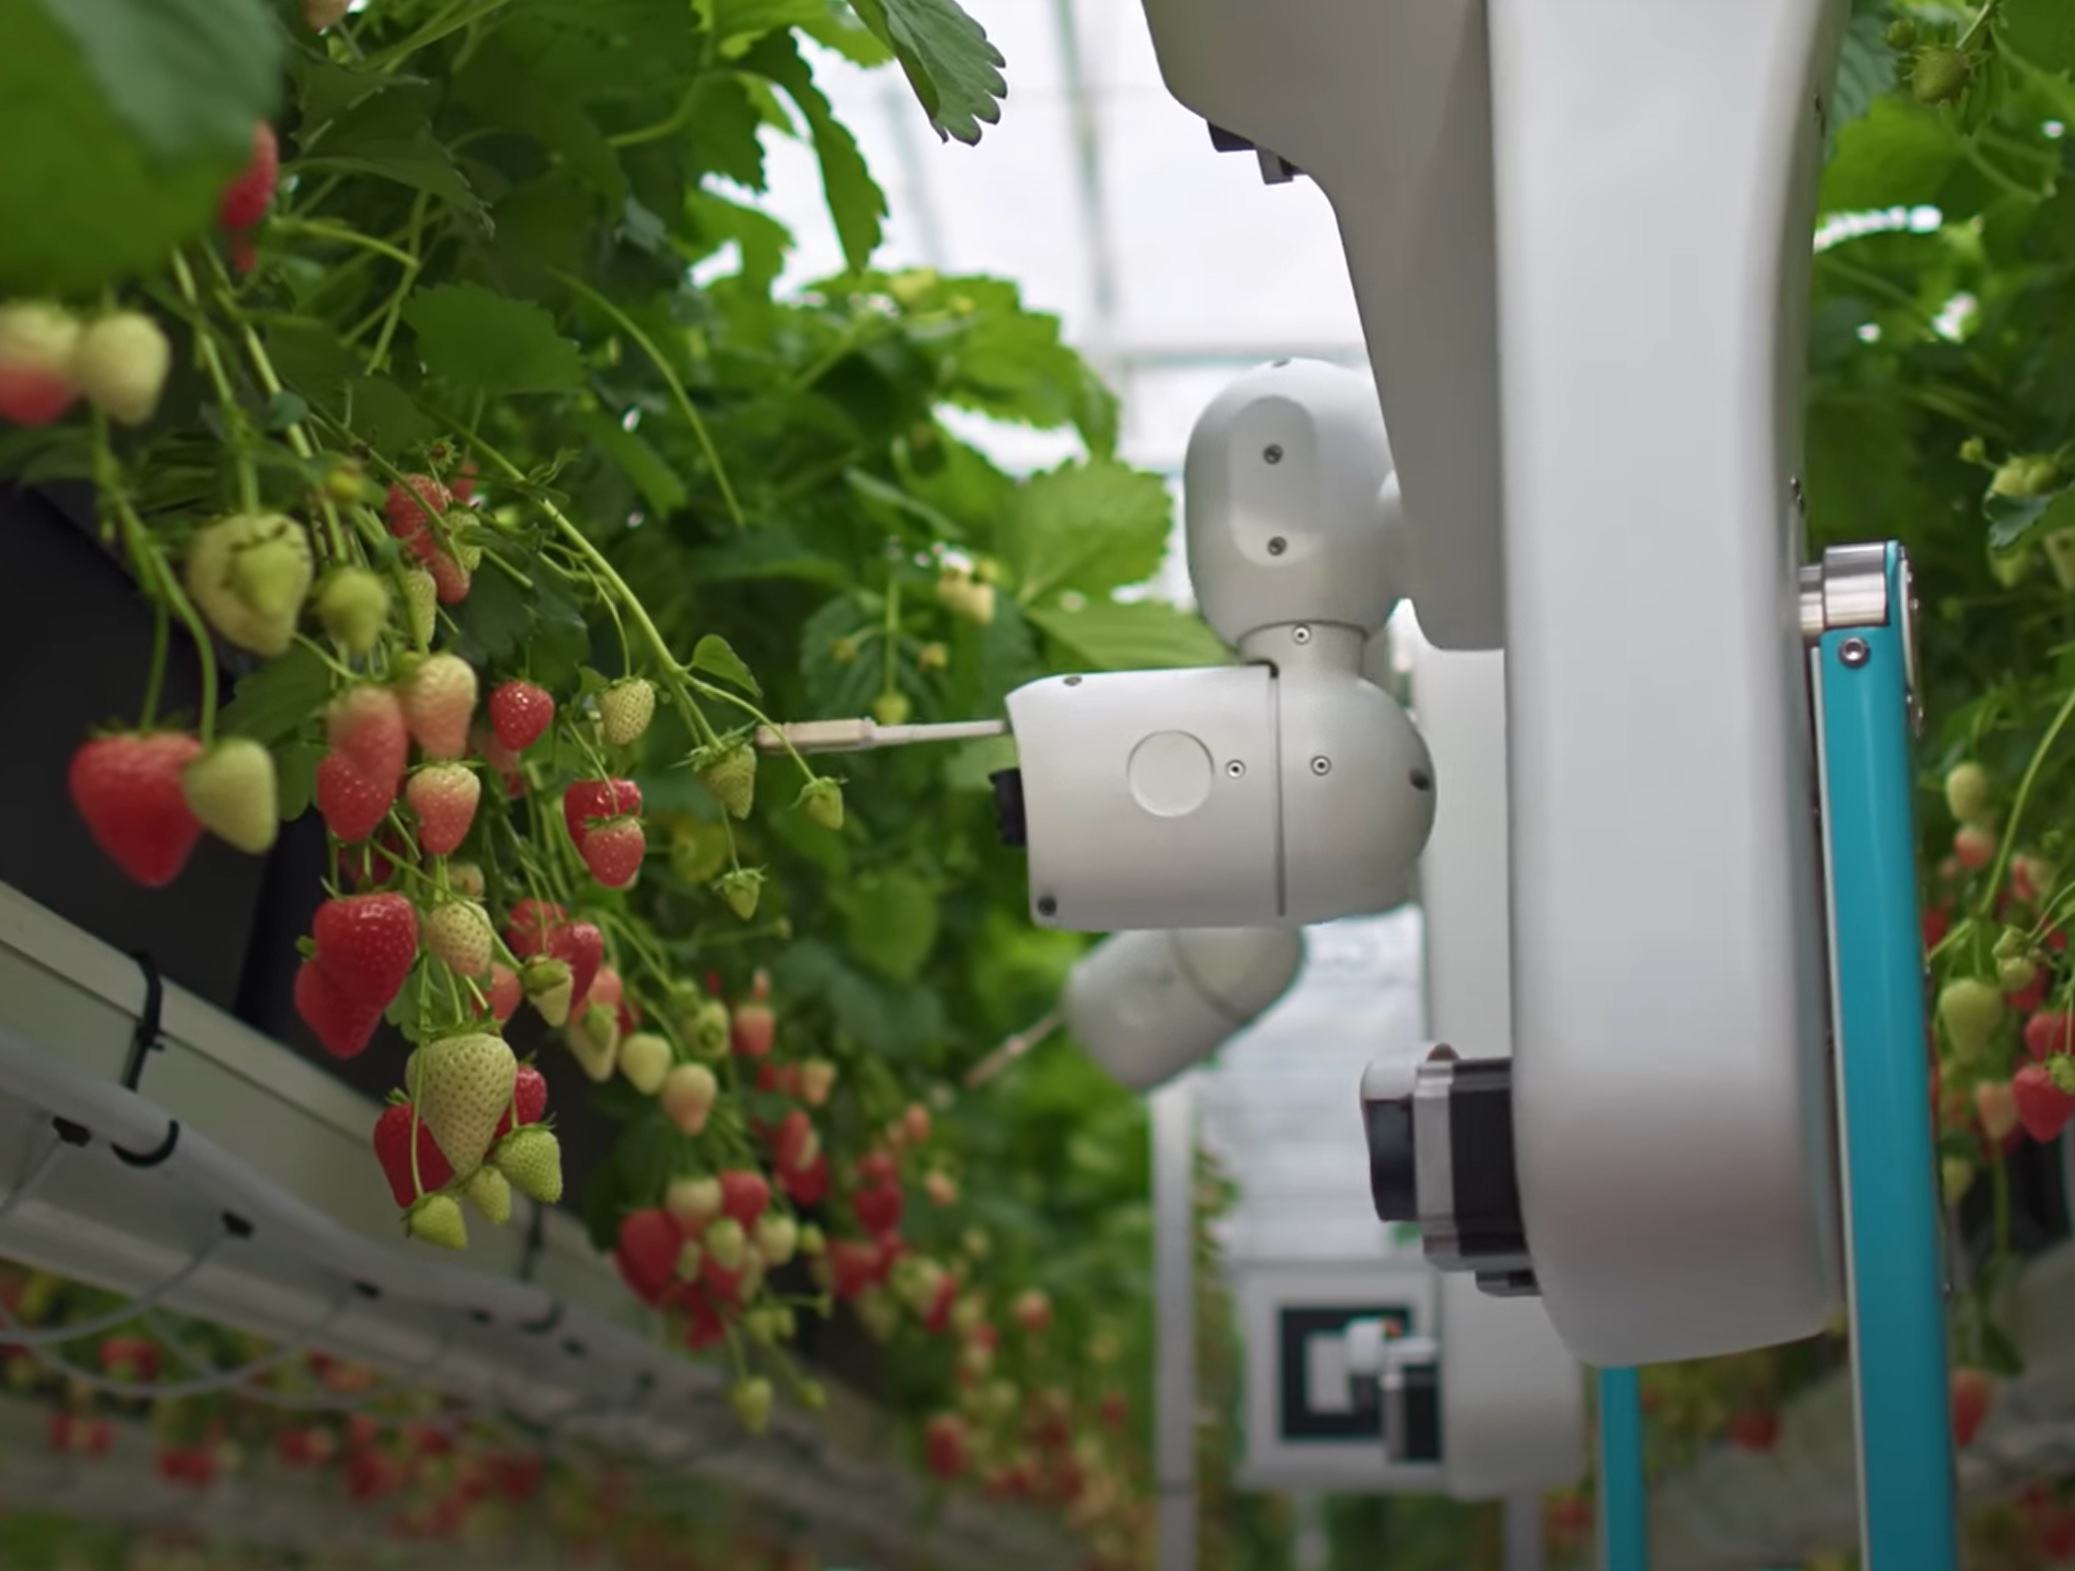
\includegraphics[scale=0.7]{image/dogtooth.jpg}
\caption{Dogtooth's robotic strawberry harvester\cite{RwhHvBJPPy4tjYjk}}
\end{center}
\end{figure}
\newpage


\subsection{Shanghai's university citrus picker}
\label{subsec:4}

Shanghai's university department of mechatronics developed a citrus picking robot \cite{9515884}. It picks citruses with over 90 \% success rate. With this achieved success rate, the robot is getting closer to the commercial goal. With a design similar to Dogtooh's robot, it uses a logical flowchart as demonstrated in picture No. 8.  Although both robots possess a robotic arm mounted on a lifting platform, the citrus picker only offers 4 DOF. It also uses 3D image processing, although without additional light sources, which implies that the robot can be used only during the day. Nevertheless, the fact that a small university team can construct and program a functional robotic harvester for citrus fruits shows that this surely is the future of agriculture. 

\bigskip
\begin{figure}[h]
\begin{center}
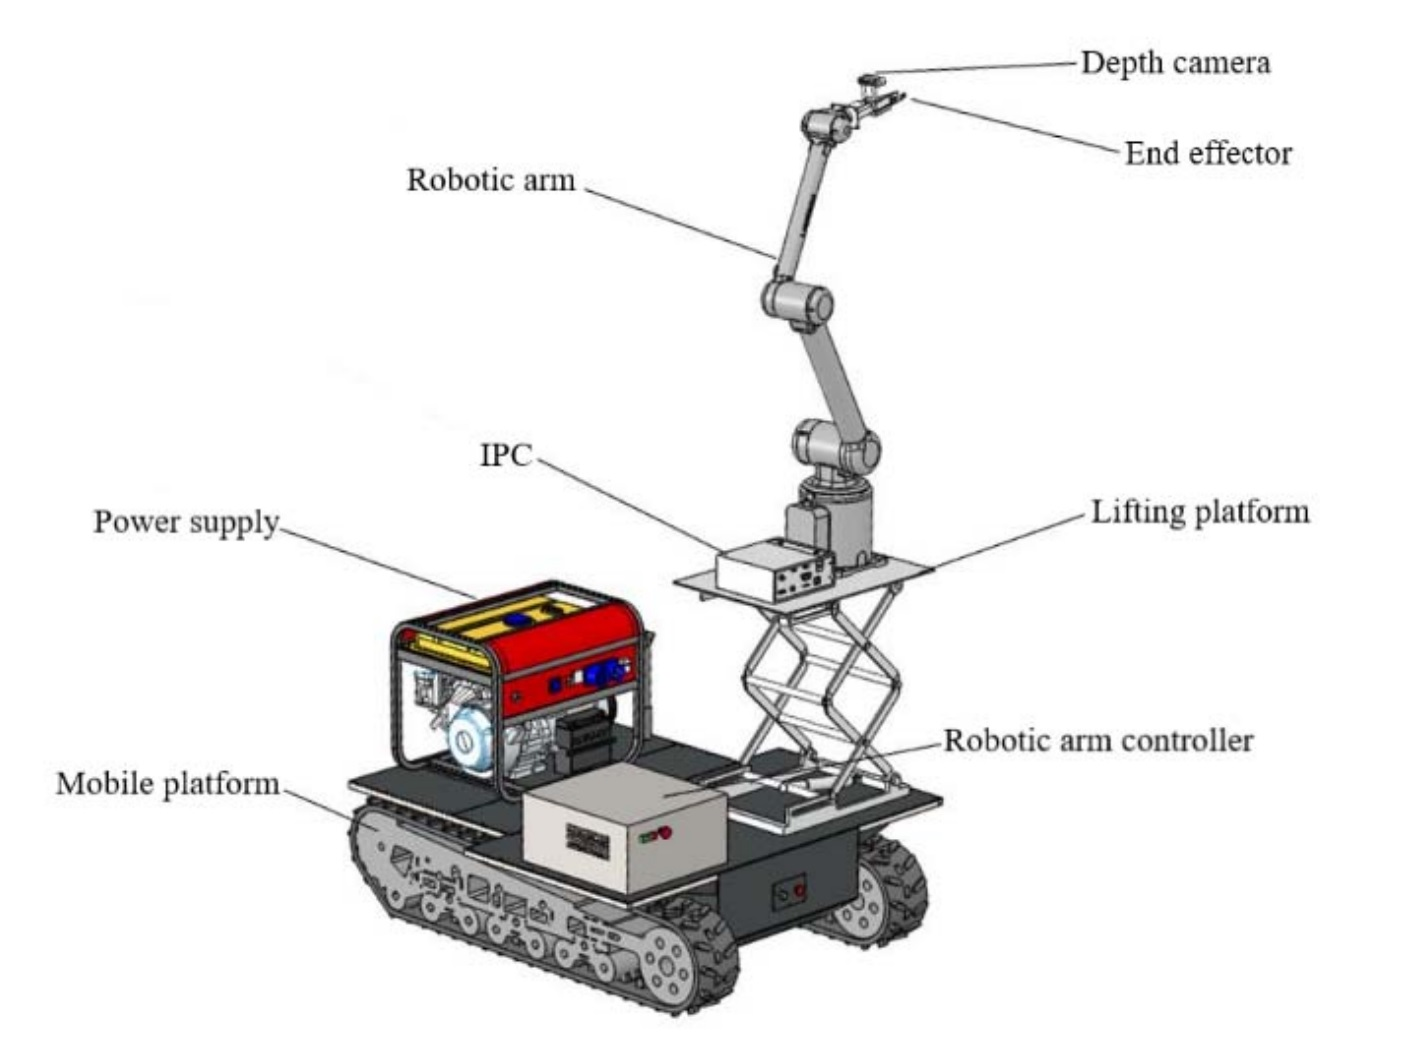
\includegraphics[scale=0.7]{image/shanghai.jpg}
\caption{Shaghai's university robotic citrus harvester\cite{9515884}}
\end{center}
\end{figure}

\bigskip
\begin{figure}[h]
\begin{center}
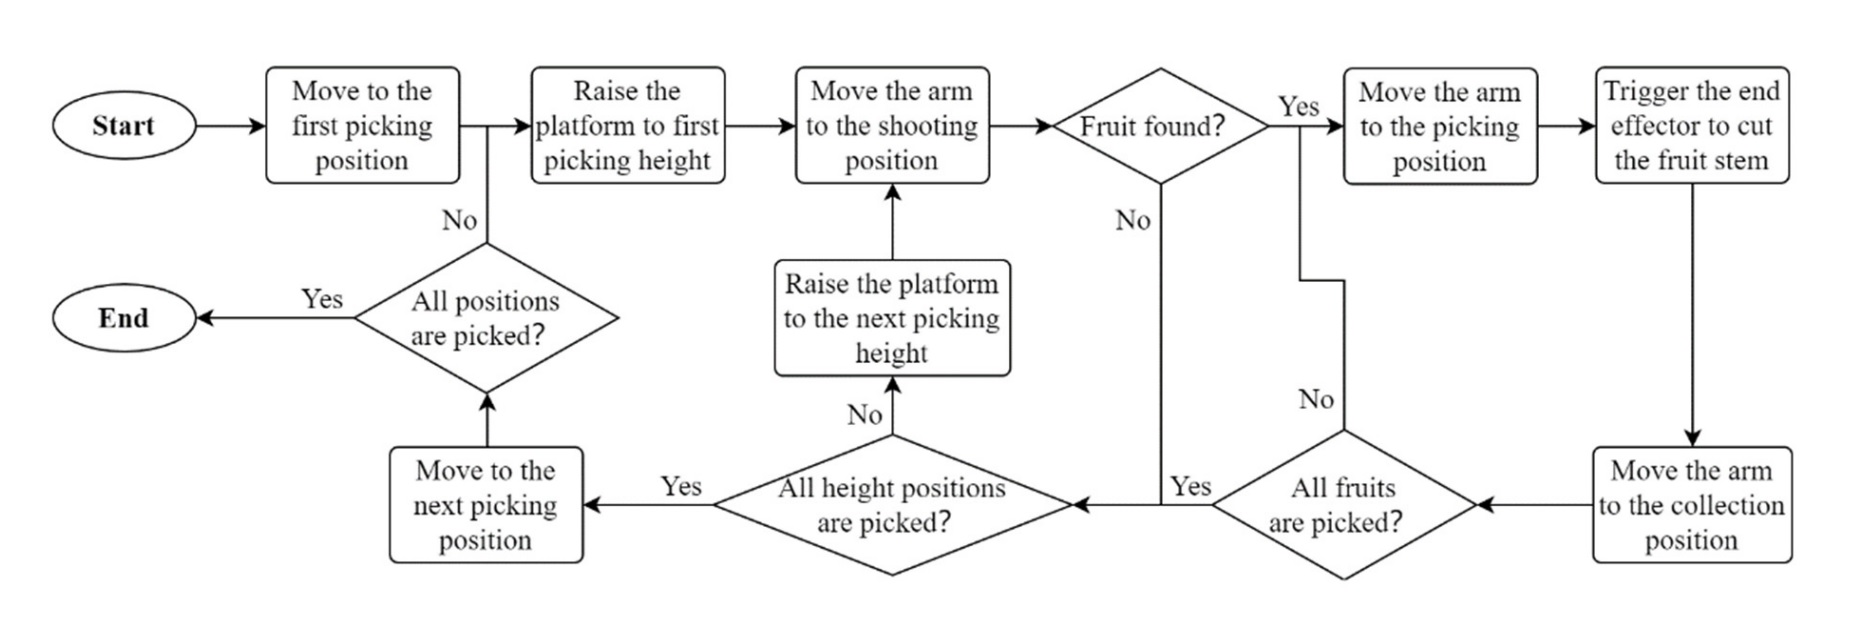
\includegraphics[scale=0.7]{image/flowchart.jpg}
\caption{Shaghai's university logical flowchart\cite{9515884}}
\end{center}
\end{figure}


\smallskip

\section{Conclusion}
\label{sec:5}
This paper's topic was the implementation of Industry 4.0 into agriculture. In the first part were discussed the weeding robotic machines, and secondly, the robotic harvesters were addressed. There is a huge potential for automatization in farming since as of today robots aren't commonly used on farms. Robotic technology makes it more affordable to produce food closer to the end customer, terminating the need to ship food all over the world and reducing the carbon footprint and price of food. Although there a still problems to solve, future farming needs to implement more robotic workers to be sustainable for the increasing human population.
\newpage

% References
%
\begingroup
\makeatletter
\renewcommand\section{\@startsection {section}{1}{\z@}%
                                   {-3.5ex \@plus -1ex \@minus -.2ex}%
                                   {4.5ex \@plus.2ex}%
                                   {\large\bfseries}}
\makeatother


\bibliography{references}{}
\bibliographystyle{acm}
\endgroup

\end{document}